

%src mongo lisence.


% https://www.techtarget.com/searchdatamanagement/definition/MongoDB
% jotain täältä. tämä tosin sanoo että on open source joka ei oo sinänsä totta
% sitaatti 28.5


%mongo website and repo
% 5.6

%https://www.mongodb.com/docs/manual/core/document/
%json bson, document format
% 5.6

%https://www.techtarget.com/searchdatamanagement/definition/MongoDB
% performance and availability
% 5.6

%https://www.mongodb.com/resources/products/fundamentals/why-use-mongodb
%used alot
% 5.6




MongoDB on NoSQL (eng "non sql"{} tai "not only sql"{}) dokumenttipohjainen tietokannan hallintaohjelma,
joka on MongoDB Inc:in valmistama ja ylläpitämä.
Se on suunniteltu käsittelemään suuria määriä strukturoimatonta dataa,
ja se tarjoaa suorituskykyisen, käytettävän ja skaalautuvan\labciteend{alexander23}
\medskip




MongoDB tallentaa tiedot joustaviin, JSON-tyyppisiin dokumentteihin, 
joka tarkoittaa, että kentät voivat vaihdella dokumentista toiseen ja tietorakennetta voidaan muuttaa ajan myötä. \labcite{mongodb24a}
Tätä tietokantajärjestelmää käytetään laajalti nykyaikaisissa sovelluksissa, 
sillä se pystyy hallitsemaan erityyppisiä tietoja ilman kiinteää skeemaa\labciteend{mongodb24b}
\medskip



\subsubsection{NoSql dokumentti -tietokannnan rakenne}




Relaatiotietokannat järjestävät tiedot taulukoihin,
joissa kukin taulukko koostuu riveistä, jotka sisältävät useita sarakkeita.
Kukin rivi edustaa yhtä kokonaisuutta tai tietuetta, ja sarakkeet määrittelevät kyseisen kokonaisuuden eri attribuutit.
Nämä taulukot on usein yhdistetty toisiinsa pää- ja vierasavaimilla,
jotka varmistavat suhteet ja ylläpitävät tietojen eheyttä koko tietokannassa.\labcite{mongodb24c}
\medskip

Sen sijaan MongoDB jäsentää tiedot kokoelmiksi.
Kukin kokoelma on samanlainen kuin relaatiotietokannan taulukko,
mutta rivien sijasta MongoDB käyttää dokumentteja tietojen tallentamiseen.
% vertailee kuulostaa jotenkin oudolta
Kuvassa \nextImageCount{} on kaavio MongoDB:n rakenteesta. 
Nämä dokumentit ovat joustavia ja sisältävät objekteja.
Toisin kuin relaatiotietokannat, MongoDB ei vaadi kiinteää skeemaa, mikä tarkoittaa, 
että jokaisella kokoelman asiakirjalla voi olla erilainen rakenne.\labcite{mongodb24c}
\medskip

\bigskip
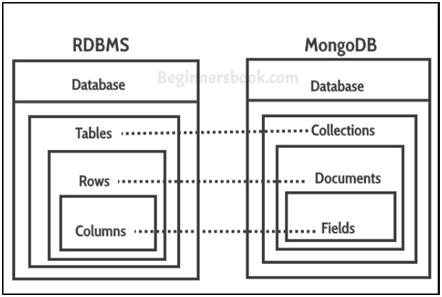
\includegraphics{src/public/oppar/mongodb-structure.jpg} \\
Kuva \getImgCount. MongoDB:n rakenne\labimgcite{lamba18}
\medskip


Dokumenttitietokannat sisältävät datan jossain standardisoidussa formaatissa kuten XML, YAML, JSON ym.
Dokumentit vastaavat karkeasti objektia, eikä niitten pidä sitoutua mihinkään standardi skeemaan, 
eikä niillä tarvitse olla samoja kenttiä.\labcite{mongodb24c}
\medskip


MongoDB tallettaa tiedot BSON muodossa, joka on binäärinen JSON formaatista.
Tietokannasta dokumentteja voi hakea niiden uniikkien tunnisteiden tai sisällön arvojen perusteella.\labcite{mongodb24a}
\medskip






\subsubsection{Skaalautuminen}

%lenove sitaatit on fine paitsi ensimmäisessä lukee jotain outoo


%https://www.lenovo.com/us/en/glossary/scalling/
%6.6

Skaalautumisella tarkoitetaan sovelluksen, järjestelmän tai infrastruktuurin
mahdollisuutta hallita kasvavaa määrää dataa, käyttäjiä tai kuormaa ilman että suorituskyky tai vakaus laskisi.
Skaalautuminen on tärkeää, kun sovelluksen käyttäjämäärä kasvaa, sillä sen pitää pystyä käsittelemään kasvavaa kuormaa.
Ilman skaalautumista järjestelmästä voi tulla hidas tai se voi johtaa seisokkiaikaan.\labcite{lenovo}
\medskip

Vertikaalisella skaalautumisella tarkoitetaan yksittäisen palvelimen tai järjestelmän olemassa olevien resurssien kehittämistä, 
kuten keskusmuistin tai prosessorin päivitystä, parantaen järjestelmän suorituskykyä.\labcite{lenovo}
%mtextPP
\medskip

Horisontaaliskaalaus käsittää koneiden ja järjestelmien lisäämistä, niin että ne pystyvät jakamaan kuorman usean palvelimen välillä.
Tämä tuo myös lisäturvaa, sillä jos järjestelmä tai sovellus kaatuu palvelinvian takia, 
toissiainen palvelin voi siirtyä ensisisijaiseksi palvelimeksi. \labcite{lenovo}
Mongodb skaalautuminen perustuu replikointi- ja shardausominaisuuksiin, jotka toimivat horisontaalisella skaalausperiaatteella\labciteend{mongodb24d} 
\medskip




MongoDB replikointi antaa mahdollisuuden tehdä varmuuskopioita tietokannasta ja säilyttää niitä eri palvelimilla.
Nämä varmuuskopiot voidaan käyttöönottaa, jos ensisijainen tietokanta kaatuu. 
Kaaviossa 1 näkyy esimerkki replikoinnin toiminnasta. 
Asiakassovellus (eng client application) lähettää kaikki kirjoitus- ja lukuoperaatiot ensisijaiselle tietokannalle, 
Ensisijainen tietokanta jakaa kaikki kirjoitusohjeet muille toissijaisille kopioille pitäen ne ajan tasalla.
Jos ensisijainen tietokanta kaatuu tai sammuu, jostain toissijaisesta kopiotietokannasta tulee uusi ensisijainen tietokanta.
Tämä kasvattaa luotettavuutta sillä, jos olisi vain yksi tietokanta, sen kaatuminen lakkauttaisi sovelluksen toiminnan. \labcite{mongodb24e}
\medskip
\bigskip

\includesvg[width = 10cm]{./src/public/oppar/mongoreplication.svg}\\
Kaavio\getChartCount{}. Replikointi-malli \labimgcite{mongodb24e}
\medskip



MongoDB sharding antaa mahdollisuuden jakaa itse tietokanta useaan osaan ja jakaa jokainen palanen erikseen eri palvelimelle.
Nämä pienemmät palat ovat "shardeja"{} ja ovat itsenäisiä osia kokonaisesta tietokannasta.\labcite{kinsta23}
Tämä on hyödyllinen, kun yhdellä palvelimella tulee ongelmia suuren tietomäärän kanssa.
Kaaviossa 2 näkyy shard klusterin toimintaperiaate ja siihen kuuluvat komponentit. \labcite{mongodb24f}
\medskip


% onko tämä kaavio vai kuva ja mitä väliä tai eroa

\bigskip
\includesvg[width = 10 cm]{./src/public/oppar/mongosharding.svg}\\
Kaavio\getChartCount{}. Sharding-malli \labimgcite{mongodb24g}
\medskip


%mongos tai reitittimen pitää vaihtaa sillä se ei ole mongos tai se on sama asia


%operaatiot parempi selitys
Kaavion 2 reitittimen (eng Router) tehtävänä on reitittää tietokantaoperaatiot oikeille shardeille käyttäen konfiguraatiopalvelimelta saatua metadataa.
Asiakassovellus on yhteydessä mongos:siin ja se toimii rapapintana käyttäjän ja shardien välillä. 
Kun asiakassovellus lähettää kyselyn tietokantaan, reititin kysyy konfigurointipalvelimelta (eng config server) millä shardeilla on kyseinen data. 
Tämän jälkeen mongos voi reitittää kyselyn shardille ja palauttaa vastauksen asiakassovellukselle.\labcite{mongodb24h}
\medskip

%asiakieli
Shard on tietokantapalvelin, joka sisältää osan koko tietokannasta.
Itse shardejen pitää olla replikasettejä.
Tämä tuo lisäturvaa datan hakuun, sillä jos shardin ensisijainen kanta kaatuu voi toissijainen kopio ottaa sen roolin. \labcite{mongodb24i}
\medskip



Konfigurointipalvelin sisältää asetuksia ja metadataa klusterista,
kuten tietoja mitkä shardit ovat olemassa, mikä on shardin tila,
yksityiskohtia siitä mitkä osat tietokannasta on tallennettu mihinkin shardeihin
ja tietoja osien tasapainottamisesta shardien välillä.
Konfigurointipalvelin on myös vastuussa shardien kuorman tasapainottamisesta ja se varmistaa jakautumisen.\labcite{mongodb24j}








